% !TEX root = DesignDocument.tex


\chapter{Sprint Results and Prototypes}

This chapter discusses the results of each sprint and documents the evolving product. It covers the decisions and progress made in our 2D Robot Simulator during the first semester of our Senior Design class and is organized by Sprints, ranging from the zeroth sprint to the sixth.    

\section{Sprint 0 Report}
All work before Sept. 21st
\subsection{Sprint Backlog}

The backlog for the zeroth sprint consisted of choosing a physics engine, setting up all team members with Ubuntu version 16.04 and ROS, and examining the STDR 2D Robot Simulator for possible use. In sprint zero, we also decided to use Git and Trello for repositories and user stories.

\begin{itemize}
	\item Set up team members in Ubuntu environment
	\item Decide whether or not to use STDR simualtor
	\item Determine development tools 
\end{itemize}

\subsection{Deliverable}

The client initially requested that we alter the functionality of the existing 2D Robot Simulator called STDR. During sprint zero, however, the team established that it would be more effective to move toward the client's change requests by starting a new software entirely. The STDR was used for reference and to assist in setting up our architecture such that it would be more versatile and allow for future plug-ins.

\begin{itemize}
	\item Team research (MVP)
	\begin{itemize}
		\item Decision to start project from scratch rather than alter STDR simualtor
		\item Box2D as physics engine
		\item QT Creator as IDE
	\end{itemize}
	\item Environment setup
	\begin{itemize}
		\item Ubuntu v 16.04 
		\item ROS kinetic
	\end{itemize}
\end{itemize}

\subsection{Results of testing}

In this sprint, the team decided to use QT Creator as a development environment and Box2D as a physics engine, which we decided had enough options to get what our product needed without going overboard on physics capabilities we would never need to implement. The work load was partitioned into four parts, one for each team member, as the GUI, the world view, the physics, and the backend. The STDR was used for reference only, and team members moved forward with learning to use the tools for their partitioned sections of work.

\subsection{Successes and Failures}

Sprint zero was successful because by the end of it the team was structured, the work divided, and the environments set up such that code could be written in the preceeding sprint.

\subsection{Modifications Required}

As this was the first sprint, there were no modifications from previous sprint work or decisions. However, we veered from the initial client request to alter the STDR simulator, as we decided to start a new software from scratch which would implement the use of a physics engine and support future plug-ins.

\subsection{Sprint Review}

Sprint zero was a success in that we established Ubuntu 16.04 as an environment for our development, all team members installed necessary softwares like Qt Creator and ROS, and we met with the client to discuss software requirements.

\subsection{Sprint Retrospective}

In retrospect, the team felt very good about progress made during this sprint. We had planned to do research during the sprint, (on the STDR, architecture, IDE, physics engine, and world view widget), and by the end of the sprint we had enough user stories and information to start writing code. Therefore we exceeded our sprint zero goals and promptly set the product in motion.


\section{Sprint 1 Report}
Sept. 21st - Oct. 5th
\subsection{Sprint Backlog}

The goals for this sprint included establishing a backlog. Some examples of user stories are supporting multiple robot shapes, being able to build robots from the program, and considering physics options like sticky wheels and moving map objects. These early user stories drove the creation of wireframes in this sprint, and ultimately the choices of the architecture design and tools used.

\begin{itemize}
	\item Create backlog of user stories
	\item Create UI wireframes
	\item Begin structuring architectural layers
\end{itemize}

\subsection{Deliverable}

At our first couple of client meetings, we discussed uses and overview of the product and delivered wireframes for a product GUI as well as a world view QT widget using Qt Graphics Framework. We also had a physics demonstration which printed out vector coordinates of two objects colliding using Box2D, and one team member determined how to use Catkin to build a Qt Widgets project. It was also during this sprint that we created our software contract. The deliverables were those wireframes, examples,the contract, and a Trello backlog of user stories.

\begin{itemize}
	\item Team research applications (MVP)
	\begin{itemize}
		\item Clickable UI
		\item Physics simulation example
		\item Catkin build functionality
	\end{itemize}
	\item Tools and documentation
	\begin{itemize}
		\item First draft of software contract
		\item Trello backlog of user stories
	\end{itemize}
\end{itemize}

\subsection{Results of testing}

Testing in this sprint was indepenedent among team members: the physics member tested uses and limits of Box2D, the UI member created a clickable UI, the world view member created a QT widget, and the backend member utilized Catkin to develop an easy way to run the project. The client accepted our software contract and approved both the cliackable UI and user stories.

\subsection{Successes and Failures}

We met the sprint one goals by the end of our two-week sprint. We established a backlog of user stories on Trello and all team members created GUI wireframes which were later used to make an initial clickable GUI and ultimately an MVP in sprint four. By the end of the sprint, the work was partitioned and the beginnings of a layered software architecture had been established.

\subsection{Modifications Required}

There was little modification from the zeroth sprint to the first, except to clear up misunderstandings about specific uses of the software. For example, it was unclear during the previous sprint whether a running simulation should pause when prompted, or reset entirely. We reached the conclusion that Qt Graphics Framework should be used for the world view widget, rather than the OpenGL widget we originally planned for. The main uses remained the same.

\subsection{Sprint Review}

Sprint one was a success in that we had a compilable project by the end of it. The four wireframes produced during the sprint were discussed with the client and we decided to take a single-window approach rather than a multi-window approach. This approach was intended to make the simulator feel like a game design engine, which was deemed desirable because the main users of the application would likely be familiar with game design applications. We established a backlog based on requests given in client meetings and all team members wrote code which applied to their section of work and would ultimately become part of the MVP.

\subsection{Sprint Retrospective}

In retrospect, the team felt okay about progress made during this sprint. We had planned to have a solid round of deliverables, which we did. We established a first draft of an architecture for the software and completed our software contract without issues. The team felt that the product was moving more slowly than planned, but that that would change once an MVP was produced. We may have lacked a little in communication due to the work being clearly divided, but bi-weekly team meetings held the project's best interests together.


\section{Sprint 2 Report}
Oct. 5th - Oct. 19
\subsection{Sprint Backlog}

The backlog for sprint two was to create a minimum viable product. This goal involved finishing interfaces, integrating the world view into the UI, and spawning a robot in the world view. The product was to be written in QT Creator such as to include a tab-like design with a simulator, a robot designer, and a map designer. The spawned robot necessary for the MVP was to be run via a python script to loop in a figure-8.

\begin{itemize}
	\item Create MVP
	\item Create interfaces for partition communication
\end{itemize}

\subsection{Deliverable}

Our major deliverable for this sprint was the MVP, which we showed to the client in a demo where we ran the single spawned robot on the figure-8 python script. To accomplish this, we had some minor deliverables like finishing interfaces for the UI and physics engine, and integrating the world view with the UI menus. The robot spawned in the middle of the world view and its velocity could be directly controlled with the python script.

\begin{itemize}
	\item Minimum Viable Product (MVP)
	\begin{itemize}
		\item Spawn single robot in center of world view
		\item Robot moves via python figure-8 script
		\item Finish interfaces for physics engine
		\item Finish interfaces for UI
		\item Integrate world view widget with UI
	\end{itemize}
\end{itemize}

\subsection{Results of testing}

Testing for this sprint was "as viewed" by the team members. The UI designer tested clickability of buttons and display of neccessary menus. The physics member tested a numerical output of two objects colliding. The backend member tested the MVP with the figure-8 python script and spawning of a single robot. During this sprint, we established that our product would, for the most part, have to be tested by users. Much of the code would not be able to be unit tested due to it being UI code or having infinite input parameter options.

\subsection{Successes and Failures}

In this sprint we succeeded in producing an MVP. We  established interfaces which would later be used to communicate via slots and signals between the UI, the world view, and the physics simulator. The single robot which spawned in the center of the world view could only spawn in the center and was hard-coded to spawn once. 

\subsection{Modifications Required}

There were no modifications from the first sprint to the second because the team was focused on producing an MVP. The client was pleased with said MVP, and no requests for change were made.

\subsection{Sprint Review}

Sprint two was a success in that we produced an MVP able to simulate a single robot on the clickable UI. Though it was hard-coded and our list of deliverables was small, this paved the way for future development. The client was very pleased with our progress and pushed to move toward sprint three goals of robot rotational capabilities and the option to spawn robots in locations other than the center of the world view.

\subsection{Sprint Retrospective}

In retrospect, the team felt substantial progress was made during this sprint. We produced an MVP and had the interfaces necessary to begin setting up communication between the UI, world view, backend, and physics simulator.


\section{Sprint 3 Report}
Oct. 19th - Nov. 2nd
\subsection{Sprint Backlog}

The backlog for this sprint involved enhancing the MVP and creating our first client presentation. The MVP allowed for the spawning of a single robot in the center of the world view, so a goal in this sprint was to spawn multiple robots at random orientations and in random locations across the map. We also wanted to be able to display properties for these robots, and select and change the properties displayed.

\begin{itemize}
	\item Allow for robots spawning at non-center of map
	\item Allow for robots to rotate while moving
	\item Be able to display and change robot properties
	\item Find a way to pass shapes around threads
\end{itemize}

\subsection{Deliverable}

The deliverable for this sprint was a prototype consisting of three robots which spawned at random locations in various orientations and moved in giant figure-8's across the world view. This was paired with the addition of viewing robot properties for one of the robots. The spawned robots were hard-coded. The progress was shown as a demo in a client meeting.

\begin{itemize}
	\item Demo of new features
	\begin{itemize}
		\item Multiple robots spawning randomly on map with random orientation
		\item Robots using differential drive kinematics
		\item Python script to drive differential drive robots in figure 8
		\item Being able to see and modify properties of robot (velocity, differential drive parameters...)
	\end{itemize}
\end{itemize}

\subsection{Results of testing}
During this sprint, we made a major architectural decision based on experimentation with integrating Box2D and threads. It was determined that continuing the multi-threaded architecture would be difficult and result in many future bugs. 

\begin{itemize}
	\item Decision was made to abandon multi-threaded design.
	\begin{itemize}
		\item Box2D does not play nicely with multiple threads
		\item It is ok if the simulation lags due to all computation in one thread because eventually timestamps will be published and control code will use that rather than its own internal clock
	\end{itemize}
\end{itemize}

\subsection{Successes and Failures}

In this sprint we succeeded in improving the MVP. We were able to show the client a product where three robots spawned in random locations with random orientations and moved about the world view, sometimes collided. We failed to implement a goal of making those robots selectable such that a specific robot's properties could be set.

\subsection{Modifications Required}

There was an architectural modification in this sprint: the switch from multi-threading to a single thread. This was known to have the potential for a slower program but we justified it with ease of code and lack of bugs. We expected the lag would be a minor issue.

\subsection{Sprint Review}
Our first team presentation was successful. The client was happy with the prototypes of our MVP and improved MVP. The team felt that good progress was made and despite the delay of switching from multi-threading to a single thread, we were able to get back on track and ready for sprint four.

\subsection{Sprint Retrospective}
In retrospect, there was no way to know without applying the project that the original multi-threaded approach wasn't going to work out. Luckily we came to this conclusion in sprint three with plenty of time to correct the architecture. Everything else in this sprint went smoothly, team coding sessions emerged as a form of integrating project partitions and proved successful.

\section{Sprint 4 Report}
Nov. 2nd - Nov. 16th
\subsection{Sprint Backlog}

The backlog for this sprint included allowing selection of robots from the world view and a side menu in the UI, implementing LIDAR and touch sensor plugins, loading of obstacle (map) files, and a prototype joystick for the UI. We also had to decide on a direction for the physics aspect of the project because the MVP involved a hard-coded robot a with specific design and we were ready to start looking at alternate robot possibilities.

\begin{itemize}
	\item Decide between kinematics and full-simulation physics
	\item Allow selection of robot from main view and UI menu
	\item Prototype joystick UI
	\item LIDAR plugin
	\item Touch sensor plugin
	\item Load obstacle files
\end{itemize}

\subsection{Deliverable}

In sprint four, we delivered the ability to select a robot from a menu in the UI and load obstacle files. The touch sensor implementation plus an obstacle file of four squares emulating a "room" assisted in confirming the correct response from collisions. We presented the physics decision to move away from the hard-coded differential drive and the client informed us of some possible changes.

\begin{itemize}
	\item Demo of new features
	\begin{itemize}
		\item Physics decision
		\item Ability to select a robot from a UI menu
		\item Ability to load obstacle files
		\item Confirmed collisions
		\item Touch sensor implementation
	\end{itemize}
\end{itemize}

\subsection{Results of testing}

In this sprint, we decided to change a few things in the project in order to reach an outcome as versatile as possible. After implementing the differential drive with collisions, we decided to rip, root, and reboot the physics aspect of the project. Loading the obstacle files required use of some of the interfaces created in sprint one.

\subsection{Successes and Failures}

Touch sensors and obstacles took longer than expected to implement and required major changes in object interfaces. As a result, the ability to select a robot by clicking its image was delayed and the LIDAR plugin was not written. The joystick prototype was not completed. The client also mentioned ROS 2 as a possible target in developing this project.

\subsection{Modifications Required}

While the touch sensor plugin was being written, it was discovered that Box2D can be leveraged to model a top-down vehicle. As a result, it was decided that this method of modeling robots should be used instead of kinematic modeling. The original robots spawned in the sprint two and three demos used a kinematic differential drive. The client warned us to watch out for possible changes from ROS to ROS 2 and we also discussed changing the foundation of differentiating between map objects and robots. We decided the product would be more useful if robots and map objects were created and treated the same way. Thus, we set out to redo the UI such that "Simulation Mode" would become a "Simulator" while "Map Mode" and "Robot Mode" would merge to become a single "Designer". This would allow for the creation of non-static map objects such as moving doors and doors with sensors. Overall, this would make the software more versatile.

\subsection{Sprint Review}

The client was again pleased with progress made. Our next target features were identified as implementing obstacles and some sort of sensor equipment so that the application could potentially be used in a class project. This along with revamping the UI, fixing the hard-coded kinematic physics, and implementing the Designer for world view objects led the direction we took moving into sprint five.

\subsection{Sprint Retrospective}

In retrospect, sprint four was pivotal as a post-MVP turning point for the product. We had enough code written to determine what was working and what was not, and made decisions that would ultimately push the product to be as versatile as possible.


\section{Sprint 5 Report}
Nov. 16th - Nov. 30th
\subsection{Sprint Backlog}

The backlog for this sprint included no programming. It was a sprint of documentation, client presentation number two, a discussion on ethics, and team evaluations.

\begin{itemize}
	\item Documentation
	\begin{itemize}
		\item Overview
		\item Project Plan
		\item Requirements
		\item Design
		\item Test Plan
		\item Prototypes
		\item Software Contract	
	\end{itemize}
	\item Presentation
	\item Ethics Quiz
	\item Team Evaluations
\end{itemize}

\subsection{Deliverable}

In sprint five, we focused on documentation catch-up. We wrote most of this document during sprint five, as well as our second client presentation, our team evaluations, and completeing a quiz on ethics in computer science.

\begin{itemize}
	\item Client presentation showcasing:
	\begin{itemize}
		\item Changes since STDR
		\item New GUI
		\item Physics decisions
		\item Future sensor implementation plans
	\end{itemize}
	\item Team evaluations
	\item Senior Design Final Documentation
	\item Ethics discussion
\end{itemize}

\subsection{Results of testing}

Our presentation was well-recieved by the audience and client alike. We decided to split up the documentation as much as possible such that the team members each wrote about sections of code they had written or architectural decisions they had made. We decided to include a side by side comparison in our presentation of our software against the STDR. This video was more effective to show differences than a dotted list would have been.

\subsection{Successes and Failures}

Our presentation was a success. The audience understood the project and we had ample imagery to show the changes we had made. We succeeded in submitting our team evaluations on time and bonded over a long discussion about the ACM code of ethics. We procrastinated a bit on the documentation but in the end, it got completed. 

\subsection{Modifications Required}

There were no major changes made during this sprint, except to shift the team's focus from coding to documentation. We had a lot of changes to make to the documentation, as we previously hadn't had all the information necessary to fill out several sections.

\subsection{Sprint Review}

The team felt that this sprint was successful despite writing no code and looking at the software itself very little. It was used mostly for reference to complete the documentation. We were able to complete all backlog items for this sprint and set up team members' tasks for the winter break.

\subsection{Sprint Retrospective}

In retrospect, sprint five was necessary and felt rushed. Writing documentation is, of course, less enjoyable than writing a 2D robot simulator and therefore we lacked some of the passion we had as a team for the previous five sprints (0-4). The ethics discussion really helped to give us all a sense of each other's priorities when it comes to developing software. Even though our software does not posess much controversy when it comes to ethics, understanding each other as individuals assisted in building a strong team connection.


\section{Sprint 6 Report}
Nov. 30th - Jan. 11th
\subsection{Sprint Backlog}

The entire Christmas break was designated to this sprint. The backlog for this sprint included fnishing the prototype joystick for the UI, adding Doxygen to the code, implementing image loading for the map, redoing the physics, loading and saving objects, LIDAR and possibly other sensors, time warping the simulation, and more documentation.

\begin{itemize}
	\item Joystick Prototype
	\item Doxygen	
	\item Image Loading
	\item New Physics
	\item Object load/save
	\item LIDAR
	\item Maybe other easy sensors
	\item Time Warp
	\item Full Spring Semester Plan Draft
\end{itemize}

\subsection{Deliverable}

In sprint six, we started a lot of features that did not get fully implemented, such as the joystick, image loading, and loading and saving world objects. User stories completed were the LIDAR and determining a plan for the remaining spring semester sprints.

\begin{itemize}
	\item New Physics
	\item Spring Semester Plan
	\item LIDAR sensor
\end{itemize}

\subsection{Results of testing}

At this point we determined our software was pretty functional in terms of the original goal. We compiled a list of new features left to implement before we started testing and collecting bugs. This list included more sensor plugins, more component plugins, the joystick control, world object designer, and saving/loading files.

\subsection{Successes and Failures}

This sprint, while slow, was successful as far as creating a plan for what remained of the project. We determined the software could not be tested by the spring semester robotics class but we would be able to write some tests for specific features. Image loading ended up being a more difficult task than anticipated due the need to break large image bodies into Box2D-compatible shapes.

\subsection{Modifications Required}

A couple decisions were made during this sprint, such as choosing not to try and test our software with the spring robotics class and also altering the physics. Some of the tasks were re-assigned and we decided on most important features to implement during the following semester.

\subsection{Sprint Review}

This sprint was successful as a planning sprint. We made a couple design decisions, worked with the client to compile a list of desired features moving forward, and assigned tasks to team members.

\subsection{Sprint Retrospective}

In retrospect, sprint six was a lax sprint that set the framework for the sprints to come. The team didn't communicate much over the break, though that was expected. Overall, it was a necessary sprint that solidified our plans for the future.

\section{Sprint 7 Report}
Jan. 11th - Jan. 25th
\subsection{Sprint Backlog}

The backlog for this sprint included finishing the joystick prototype, finishing the image loading, testing the software on Windows and ROS2, and implementing differential drive and the circle plugin.

\begin{itemize}
	\item Joystick Prototype
	\item Run on Windows
	\item Image Loading
	\item Differential Drive
	\item Circle Plugin
	\item Test with ROS2
	\item Load / Save files
\end{itemize}

\subsection{Deliverable}

In sprint seven, we focused on finishing some of the user stories started in sprint six, as well as implementing some new plugins and testing our product with different environment variables. The joystick prototype was completed and good progress was made in the realm of image loading.

\begin{itemize}
	\item Bug Fixes:
	\begin{itemize}
		\item Robot selection in active list matching green robot
		\item Properties updating when changed
		\item No NaN at start bug
		\item No crash while coloring shapes	
	\end{itemize}
	\item Project builds with ROS2
	\item Project works on Windows 10
	\item Moveable joystick window
\end{itemize}

\subsection{Results of testing}

Our product worked with ROS2 and also on Windows 10, but only for specific team members. One team member could not get the product to run on his Windows 10 despite seemingly no difference from the environment used by other team members. We discussed trying the product out on Mac OS as well, but could not find a viable machine on which to test it. It was in this sprint that we really started collecting and fixing bugs, because we finally had enough of a product to determine what was and was not working. 

\subsection{Successes and Failures}

We successfully adapted our project to run on Windows 10 and with ROS2, expanding our deployable environment requirements from strictly Unix systems, though we were not able to test it on Mac OS. Loading images as well as loading and saving files were pushed to backlog for the next sprint. The joystick was completed but not yet integrated into the software. Some bugs that hindered development were fixed.

\subsection{Modifications Required}

While there were no changes to the product architecture in this sprint, we did add in support for ROS2 and Windows 10. We had a few iterations of algorithms before solidifying a method for image triangulation. A few bugs popped up that required fixing, but they were promptly taken care of.

\subsection{Sprint Review}

The team felt that this sprint was successful because we established product compatibility with Windows 10 and ROS2. We lacked a little on implementation of new features but made headway with the joystick control and image loader as well as a couple client-requested plugins.

\subsection{Sprint Retrospective}

In retrospect, progress was slow during sprint seven as far as product development but we made good progress in expanding our client options with testing on Windows 10 and using ROS2. This will ultimately make our product more desireable in the testing and usage phases to come after this semester ends.


\section{Sprint 8 Report}
Jan. 25th - Feb. 8th
\subsection{Sprint Backlog}

The backlog for this sprint included completeing the image loading, integrating the joystick control, and implementing rectangle and ackermann steer plugins.

\begin{itemize}
	\item Image Loading
	\item Implement Ackermann steering
	\item Rectangle plugin
	\item Integrate joystick
	\item Control script for joystick
\end{itemize}

\subsection{Deliverable}

In sprint eight, we finished the image loading functionality, ackermann steering, the rectangle plugin, and controls for the joystick, which got integrated into the software. We did some backend clean-up as well that was not necessarily visible at the product frontend but left nicer source code for future developers.

\begin{itemize}
	\item Boilerplate start for image loader
	\item Simple Shape plugin
	\item UI bug to resize screen
	\item DLL fixes
	\item Clone function for world objects
	\item Joystick integrated with signals to physics models
	\item Lidar sensor
	\item Update Box2D version
	\item Rectangular robot
	\item Ackermann steering
	\item Consolidate packages for product
\end{itemize}

\subsection{Results of testing}

The joystick did not integrate as smoothly as planned, and some alterations had to be made in order to prevent a memory leak in the program. Rectangular robots and Ackermann steering both worked as planned except for the appearance of the "jello" effect, whereby the way Box2D handles welded objects made a particular robot wobble uncontrollably while moving.

\subsection{Successes and Failures}

We successfully integrated the joystick and implemented both rectangle and Ackermann plugins for the software. There was some bug fixes and code clean-up that went smoothly, such as new functions for world objects needed by the designer and enabling a logical user resize of the window. A couple issues we ran into were a minor memory leak that was fixed and the robot "jello" effect which prompted us to build in a window where users can alter robot mass settings until it no longer wobbles. The client would have preferred if the software could handle this but we decided to give default mass settings and otherwise keep it open-ended in case different users have different requirements for the individual simulations.

\subsection{Modifications Required}

Interaction between Box2D and world objects created the issue of wobbling wheels or the "jello" effect, which will have to be dealt with by users in the future via altering object mass until the desired effect is achieved. The UI was modularized by creating the mode controller object, such that the designer and simulator were controlled as mode controller objects by the main UI. This cleaned up the UI code and minimized code repetition which was getting imense with the creation of the world object and simulation designers. Other backend cleanup was implemented as well, such as DLL alterations and updating the version of our Box2D library.

\subsection{Sprint Review}

The team felt that this sprint was successful because we integrated the joystick, implemented rectangular robots and Ackermann steering, and continued to make progress with the image loader. We were happy to see that progress didn't slow too much with the transition into spring semester and we were still making strong headway with the product.

\subsection{Sprint Retrospective}

In retrospect, sprint eight took some of the pieces the team had been working on in previous sprints and brought them together. We successfully completed implementation of the joystick and the rectangle and Ackermann plugins. We came upon the issue of the "jello" effect, which we discussed with the client in later sprints to determine that it will be an ongoing issue with the software that individual users will have to play around with to obtain desired effects.

\section{Sprint 9 Report}
Feb. 8th - Feb. 22nd
\subsection{Sprint Backlog}

The backlog for this sprint included integrating the image loader, implementing the robot designer, starting a user manual, and fixing bugs that popped up during development in the previous sprints.

\begin{itemize}
	\item User Manual Documentation
	\item Integrate image loading
	\item Object Designer	
	\item Fix Joystick bugs
	\item Fix Ackermann Steer bugs
\end{itemize}

\subsection{Deliverable}

In sprint nine, we accomplished some bug fixes and integrated the image loader such that the user could choose any image, select a greyscale number, and import it into the simulation as a series of Box2D triangles. We also started discussing the user manual and things to include.

\begin{itemize}
	\item Bugs Fixed:	
	\begin{itemize}
		\item Joystick key selection
		\item Joystick sending correct numbers
		\item Ackermann steering glitch
	\end{itemize}
	\item Image loading with triangulation integrated into product
	\item Picked environment for User Manual
\end{itemize}

\subsection{Results of testing}
We found some bugs in the josytick and Ackermann steering because of our testing in this sprint, which were quickly resolved. The client decided he would like us to use Sphinx for the user manual with possible future implementation in the Senior Design class to replace LaTex.

\subsection{Successes and Failures}
Some of our implemented features required bug resolutions in this sprint, like the joystick and Ackermann steering. Map import button worked, but the images did not scale correctly. The object designer was not completed.

\subsection{Modifications Required}

In this sprint, we picked an environment for writing the user manual and integrated the image loader, which responded interestingly to some of the testing images. Because some of the images contained very curved lines and some contained very thin lines, we decided to allow the user to define a few settings that would determing how "precise" they needed the image to be once loaded into Box2D-compatible triangles. Other than that, the World Object Properties Wrapper was updated to work for both objects and components. This was necessary for modularity between the designer and the simulator when adding components to the tools lists.

\subsection{Sprint Review}

The team felt that this sprint was successful because we integrated the image loader, which the client was very pleased with, and made modifications necessary to implement the world object designer. We also started the user manual, which didn't really need to be completed until future sprints, so we felt we were still progressing with strong momentum.

\subsection{Sprint Retrospective}

In retrospect, sprint nine displayed our dwindling reservoir of new features to implement. At this point, it was basically the designer and some plugins that we had left before testing, documentation, and bug collecting would completely take over our time.

\section{Sprint 10 Report}
Feb. 22nd - Mar. 8th
\subsection{Sprint Backlog}

The backlog for this sprint included completing the world object designer, implementing file load/save, enabling the movement and rotation of objects in the world view, and fixing bugs.

\begin{itemize}
	\item Object Designer
	\item Time warping / speed button
	\item File Load / Save
	\item Rotate and Move World Objects
	\item Fix Image Loader bugs
\end{itemize}

\subsection{Deliverable}
In sprint ten, we confirmed functinoality of plugin loading, implemented rotating/moving world view objects, and worked on, but did not complete, the object designer. We also globalized World Object Component to make objects moveable on the map and fixed bugs like the program crashing while loading many world objects, objects being moveable during simulation play, lidar seeing invisible or non-colliding objects. We also got the speed button functioning just in time for the client presentation next sprint.
 
\begin{itemize}
	\item Fixed LIDAR bugs	
	\item Speed Button
	\item Added Rotate and Move World Object Tools
	\item Fix Image Loader bugs
	\item Changed Property to have distinct incoming/outgoing signals
	\item Able to build shape, sensor plugins
\end{itemize}

\subsection{Results of testing}

We were able to test the planned functionality for plugin components, which worked. The object designer worked after some modification, and we were able to export built robots to the simulator. Objects on the world view rotated and moved correctly for the most part, with some minor bugs in the designer using the rotate tool. We had to alter the signals for world object properties to the UI in order to get them updating in the backend models.

\subsection{Successes and Failures}
We successfully tested our component plugin compatibility. We also were able to fix some bugs with the lidar and image loader, and alter the properties signals to incorporate user changes in the models. During this sprint, our scrum master had to reimage his computer, which took a chunk of time out of his sprint schedule. The world object designer from the backlog did not get completed. However, we still completed most of the backlog items and made good progress in the product.

\subsection{Modifications Required}
We had to make world objects global in order to successfully get them to move on the world view. We also cleaned the makefile and debug/release flags, added epsilon checking for property values closer to 0. For the time warping, we modified the base speed of the simulation to be slower. This allowed us two levels of "faster" simulation without producing a glitchy output.

\subsection{Sprint Review}
The team felt that this sprint was successful despite the reimaging of a laptop. We were able to piece together some of the final user stories that we planned to get done before our final client presentation. Aside from the incompletion of the world object designer, which was pushed onto the next sprint.

\subsection{Sprint Retrospective}

In retrospect, sprint ten was a good preparatory sprint for the final client presentation. Much of what we got done was easy to show in a demo and thus created a more significant effect when we later showcased the progress we had made on the project.


\section{Sprint 11 Report}
Mar. 8th - Mar. 22th
\subsection{Sprint Backlog}

The backlog for this sprint included file load/save, JSON file formatting, client presentation three, integrating the world object designer, and some documentation.

\begin{itemize}
	\item Establish JSON file format
	\item Load / Save JSON files	
	\item Client Presentation showcasing:
	\begin{itemize}
		\item Named the product (finally) 
		\item Custom positioning of wheels and sensors
		\item Image Loading	
		\item Multiple drive systems
		\item Multiple sensors
		\item Various robot shapes (rectangular)
		\item Built in joystick control
	\end{itemize}
	\item Integrate Object Designer
	\item Remaining Documentation	
	\begin{itemize}
		\item Testing
		\item UI
		\item Sprints and Prototypes
		\item User Manual
	\end{itemize}
\end{itemize}

\subsection{Deliverable}
In sprint eleven, we completed the world object designer, completed simulation save/load, established our file format for world objects, divied out the remaining Documentation work, and gave our third client presentation.

\begin{itemize}
	\item World Object Designer
	\item World simulation loading
	\item Removed QSharedPointer requirement from file loader returns
	\item Client Presentation III
	\item Divided remaining Documentation work
	\item Established JSON file format and began work on load / save
\end{itemize} 


\subsection{Results of testing}
We got the designer fully integrated, added names to active objects list, altered plugin model sizes so they can be drawn in designer widgets, enabled modification of properties in the designer. To accomplish these, we had to remove the QSharedPointer requirement from file loader returns. We decided to go with a video demo for our presentation, rather than a live demo, and used the same presentation layout as with previous client presentations.

\subsection{Successes and Failures}

Our presentation was successful. The client and class were pleased with our progress and we were finally able to show some variation in the robots we were simulating, like a rectanglular robot with Ackermann steering. We successfully integrated the world object designer, although not in time to include it in the presentation. Some of the save/load operations we were working on also did not get implemented in time for the presentation.

\subsection{Modifications Required}
We had no major modifications during this sprint, aside from removing QSharedPointers and deciding on a file format for world objects. The object designer was finally integrated so a few bugs popped up with that, which didn't get fixed until sprint twelve.

\subsection{Sprint Review}
The team felt that this sprint was successful. We gave a good presentation, other than the fact that our lack of testing reflected poorly, and continued to make progress with the final product features. The client was happy with our work and we were almost at a point of completely switching over from development to bugs and documentation.

\subsection{Sprint Retrospective}

In retrospect, sprint eleven was where our early design decisions for flexibility and expansion really started to show. We were able to create plugins for some demo robots and actually use them in the simulation. We also gave a good final presentation to showcase this and successfully finished the last major development feature: the world object designer.


\section{Sprint 12 Report}
Mar. 22th - Apr. 5th
\subsection{Sprint Backlog}
The backlog for this sprint included fixing bugs, implementing quick save/quick load, documentation, design fair poster board, and finishing up the load/save file operations.

\begin{itemize}
	\item Fix UI Bugs
	\begin{itemize}
		\item Name and Type prompt for exported robots
		\item Black borders around tool widgets
		\item Icon Reselections
	\end{itemize}
	\item Quick Save/ Quick Load
	\item Load / Save World Object Buttons
	\item Load / Save Simulation Buttons
	\item Documentation
	\item Design Fair Preparations
	\item Write unit tests
	\item Add to bugs backlog
\end{itemize}

\subsection{Deliverable}
In sprint twelve, we fixed some glaring bugs, changed the icons to all fall under one license, created some example robot files, implemented quick save/quick load, designed our board for the fair, and completed the file load/save functionality. We also removed the default robots from the simulator. Not a lot of documentation got done, so we pushed most of that onto backlog for the next sprint.

\begin{itemize}
	\item Fixed UI Bugs
	\item Solidified icon licensing
	\item Example robot files
	\item Fixed MSVC compile errors
	\item Implemented Quick Save/ Quick Load
	\item Finalized Load /Save World Objects and Simulations
	\item Design Fair Board and Q/A list
\end{itemize}

\subsection{Results of testing}
We completed our design fair board, deciding to go with a 3x3 partition of information with an entire row of images showcasing our product. In terms of the product itself, we fixed some bugs with the UI, which were mostly inconsistent dialogue boxes. We changed some icons such that icons used in the software are taken from Everaldo Coelho's "Crystal Project Icons" (http://www.everaldo.com CONTACT: everaldo@everaldo.com) under the LGPL license (https://www.gnu.org/licenses/lgpl.html). Example robot files were created to test some features like file loading and also for user convenience. There was a compile error fix and all file loading/saving was completed during this sprint.

\subsection{Successes and Failures}
In sprint twelve, we successfully created a design fair board, implemented quick save/quick load, fixed bugs/compile errors, and finalized file save/load. With our scrum master out of the country for much of this sprint, we didn't grow our bug backlog or unit tests as much as we would have liked.

\subsection{Modifications Required}
We had a couple feature modifications during this sprint, including fixes for some bugs and a compilation error. It was during this sprint that the client requested quick save/quick load as a feature to complement a simulation restart. This was in the case of a user wanting to start the simulation from a specified state, rather than using the restart button, which would reload the simulation from file. Quick save/load was implemented using a temporary file.

\subsection{Sprint Review}
The team felt that this sprint was successful despite being a little slow, which we attribute to design fair preparations and being down one teammate. We finished up the requested features and started to shift to completing the documentation.

\subsection{Sprint Retrospective}

In retrospect, sprint twelve was the last development sprint. We decided to declare a thirteenth sprint, but not for the product development so much as the documentation, testing, and bug backlog. 

\section{Sprint 13 Report}
Apr. 5th - Apr. 26th
\subsection{Sprint Backlog}

The backlog for this sprint included adding to the bug backlog, finishing the documentation, and attending the design fair.

\begin{itemize}
	\item Bug Backlog
	\item Documentation		
	\begin{itemize}
		\item Sprints and Prototypes
		\item Testing
		\item UI
		\item User Documentation
	\end{itemize}
	\item Design Fair	
	\begin{itemize}
    	\item Poster board
    	\item Possible Q/A
    	\item Presentation at fair
	\end{itemize}
	\item Product Finalization
\end{itemize}

\subsection{Deliverable}

Deliverables for this sprint included some documentation, a bug backlog, and the preparation and presentation of the design fair. 

\begin{itemize}
	\item Bug Backlog Expanded
	\item Documentation	Additions	
	\begin{itemize}
		\item Sprints
		\item Testing
		\item UI Architecture
		\item User Documentation
		\item Doxygen
	\end{itemize}
	\item Design Fair	
	\begin{itemize}
    	\item Poster board
    	\item Q/A with guests
    	\item Video of product
	\end{itemize}
	\item Tests
\end{itemize}

\subsection{Results of testing}
In sprint thirteen, we accomplished everything needed to finalize the product for the purpose of our senior design class. The design fair was a success, despite the error that kept us from doing our joystick demo as planned. People were enthusiastic about our software and the faculty scorers were impressed, though one suggested some possible testing displays that would have improved our presentation. We finishd our product documentation and wrote some tests.

\subsection{Successes and Failures}
We succeeded in completeing our documentation, writing tests, expanding the bug backlog, and presenting well at the design fair. One failure of this sprint, however, was in communication before the design fair because with our scrum master out of the country we were unable to utilize our intended joystick demo. Despite this, people enjoyed our presentation and gained interest in the RoboScience Simulator for the board, the video display, and the engaging conversations we held about the purpose of our software.

\subsection{Modifications Required}
In the final sprint, we did not change anything in our design and implementation plan. We came up with some new test cases, but that was planned, and altered our documentation to reflect changes made during the previous semester's sprints, (since sprint six).

\subsection{Sprint Review}
The team felt good about this sprint, as well as this project. We felt that we accomplished a good amount for the time given and we had good communication throughout the development cycle. We were all a little sad about not getting our joysticks working for the design fair, but with how well the rest of the presentation went it wasn't too much of an issue.

\subsection{Sprint Retrospective}
In retrospect, sprint thirteen was a successful wrap to our project. We had all our development finished before the sprint began and had only to work on our documentation and design fair presentation. We felt that the design fair was successful and we had designed the RoboScience Simulator in a flexible way such that it could be used and altered by the public with minimal stress. In the weeks following the official release on GitHub, I'm sure we will all be watching to see how it goes.

\section{Prototypes}

\subsection{Early Architecture Design}
Early implementations of the project did not have as clearly defined data types and separation between the different sections of the project. Figure \ref{fig:prototypediagram} shows an early block diagram of the architecture. 

\begin{figure}[h]
	\centering
	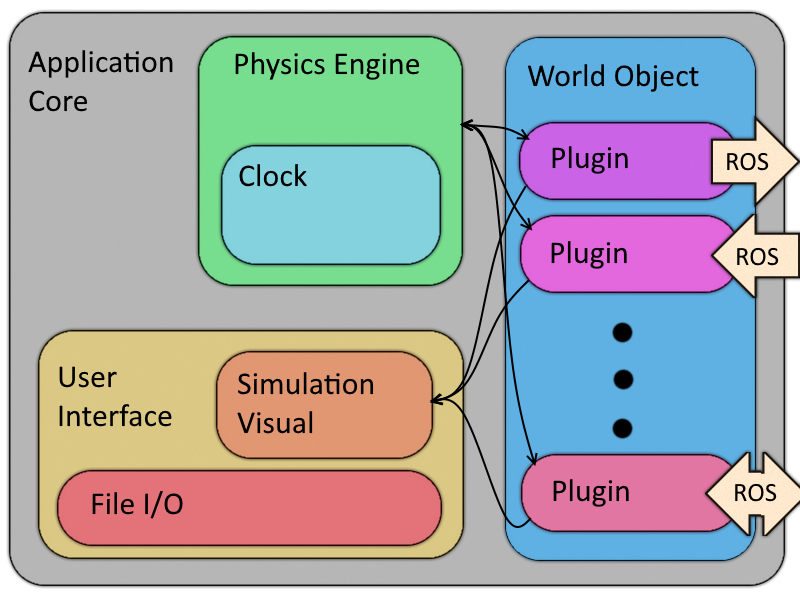
\includegraphics[width=0.75\textwidth]{./images_design/sysarch}
	\caption{Early block diagram of the project architecture. Compare to the current version in Figure \ref{fig:systemdiagram}}
	\label{fig:prototypediagram}
\end{figure}

\subsection{STDR Simulator}

The STDR was the original 2D robot simulator the client was using in robotics classes. The team was asked to modify it as our senior design project, but after careful deliberation we decided it would be more effective to start a new project. Visible in the figure below is a simulation of two robots implementing many sensors to navigate a maze.

\begin{figure}[!htb]
	\begin{center}
		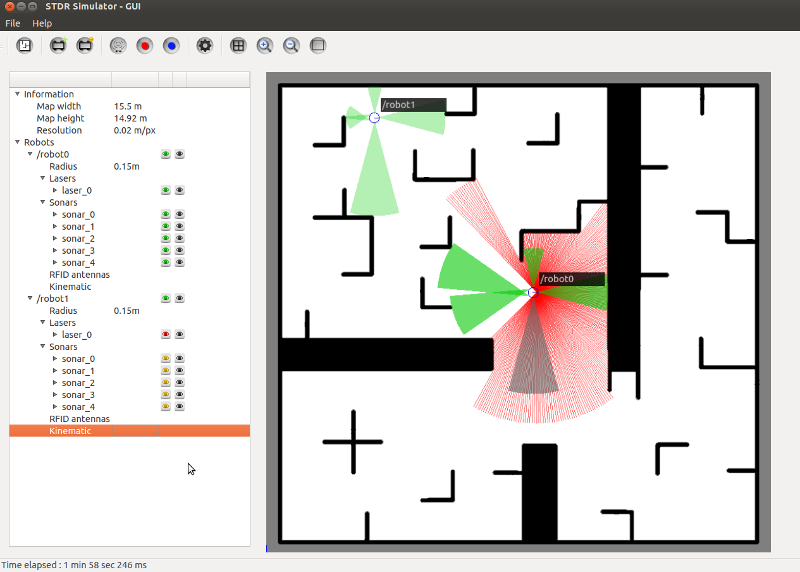
\includegraphics[width=0.75\textwidth]{./Images/Sprint0_STDR}
	\end{center}
	\caption{The original STDR 2D robot simulator, which the client initially wanted the team to modify.  \label{stdr}}
\end{figure}

\subsection{Clickable UI}

The clickable UI prototype consisted of buttons and slots partitioned into three sections: Simulation Mode, Map Mode, and Robot Mode. The intention during production of this prototype was to emulate a video game designer and produce a visual deliverable for the client. A blank black widget is visible where the world view is supposed to be, as this prototype did not have the world view integrated into the UI.\newline\newline\newline
\newline\newline\newline
\newline\newline\newline

\begin{figure}[H]
	\begin{center}
		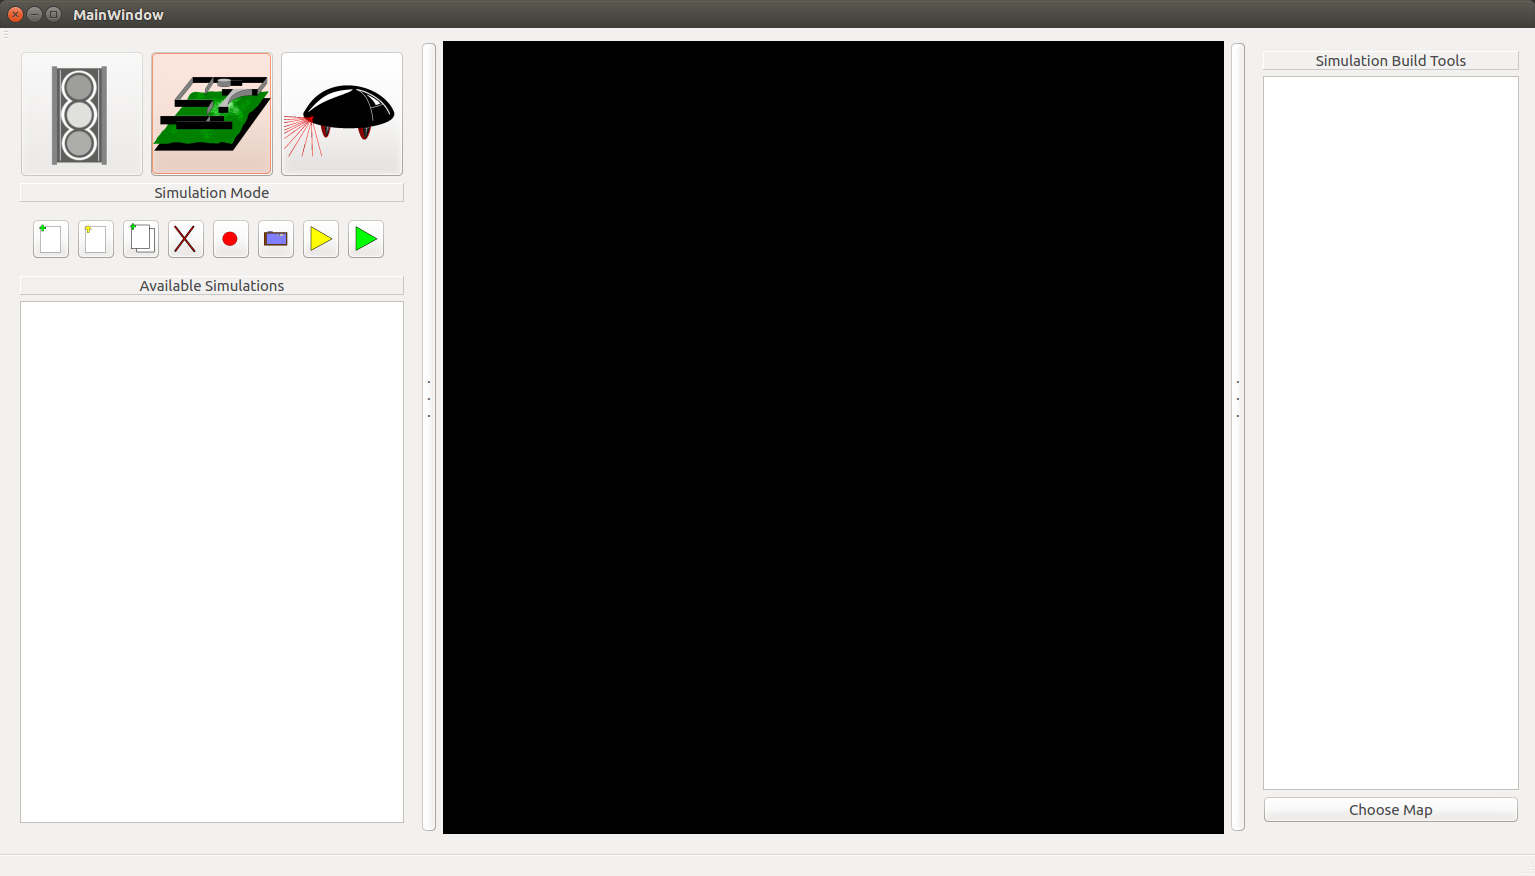
\includegraphics[width=0.60\textwidth]{./Images/Sprint1_clickableUI_SimulationMode}
	\end{center}
	\caption{The clickable UI with Simulation Mode, currently set in Simulation Mode.  \label{clickableuisimulation}}
\end{figure}

\begin{figure}[H]
	\begin{center}
		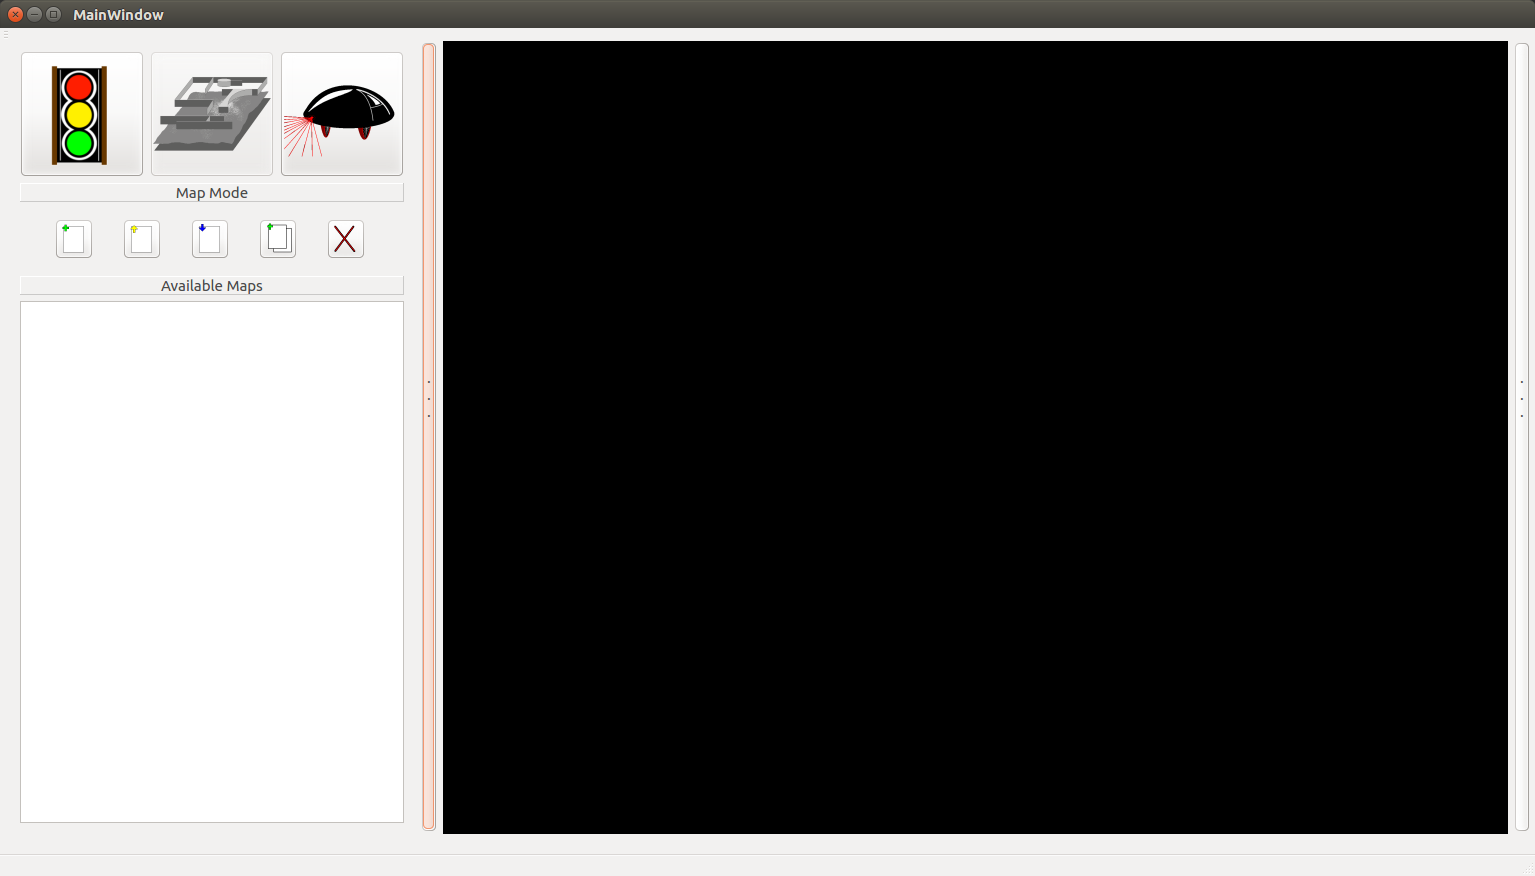
\includegraphics[width=0.60\textwidth]{./Images/Sprint1_clickableUI_MapMode}
	\end{center}
	\caption{The clickable UI, currently set in Map Mode. \label{clickableuimap}}
\end{figure}

\begin{figure}[H]
	\begin{center}
		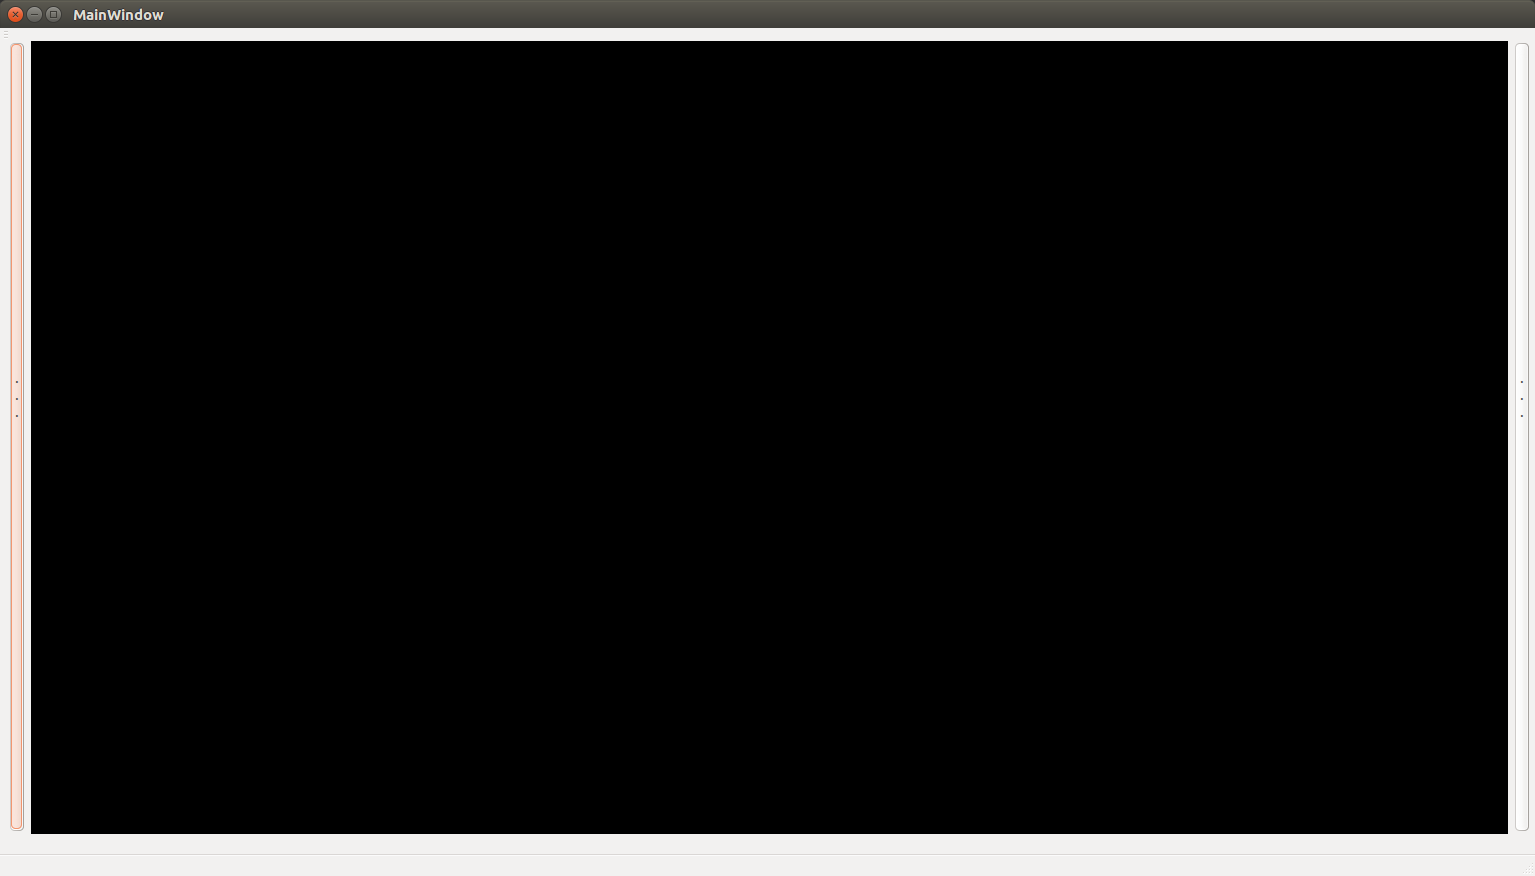
\includegraphics[width=0.60\textwidth]{./Images/Sprint1_clickableUI_NoMenus}
	\end{center}
	\caption{The clickable UI with side menus "minimized", a design decision based on the possible need to view robots moving on a larger map more easily. \label{clickableuinomenus}}
\end{figure}

\subsection{Modified MVP}

The original MVP consisted of a single robot spawning in the center of the world view and moving in a figure-8 with no obstacles to collide with. Here is the modified MVP from sprint four, in which three robots get spawned randomly throughout the world view. Also pictured is the "room" made up of four map objects which are static squares loaded from an obstacle file. Properties for one of the robots are listed on the menu to the left.

\begin{figure}[!htb]
	\begin{center}
		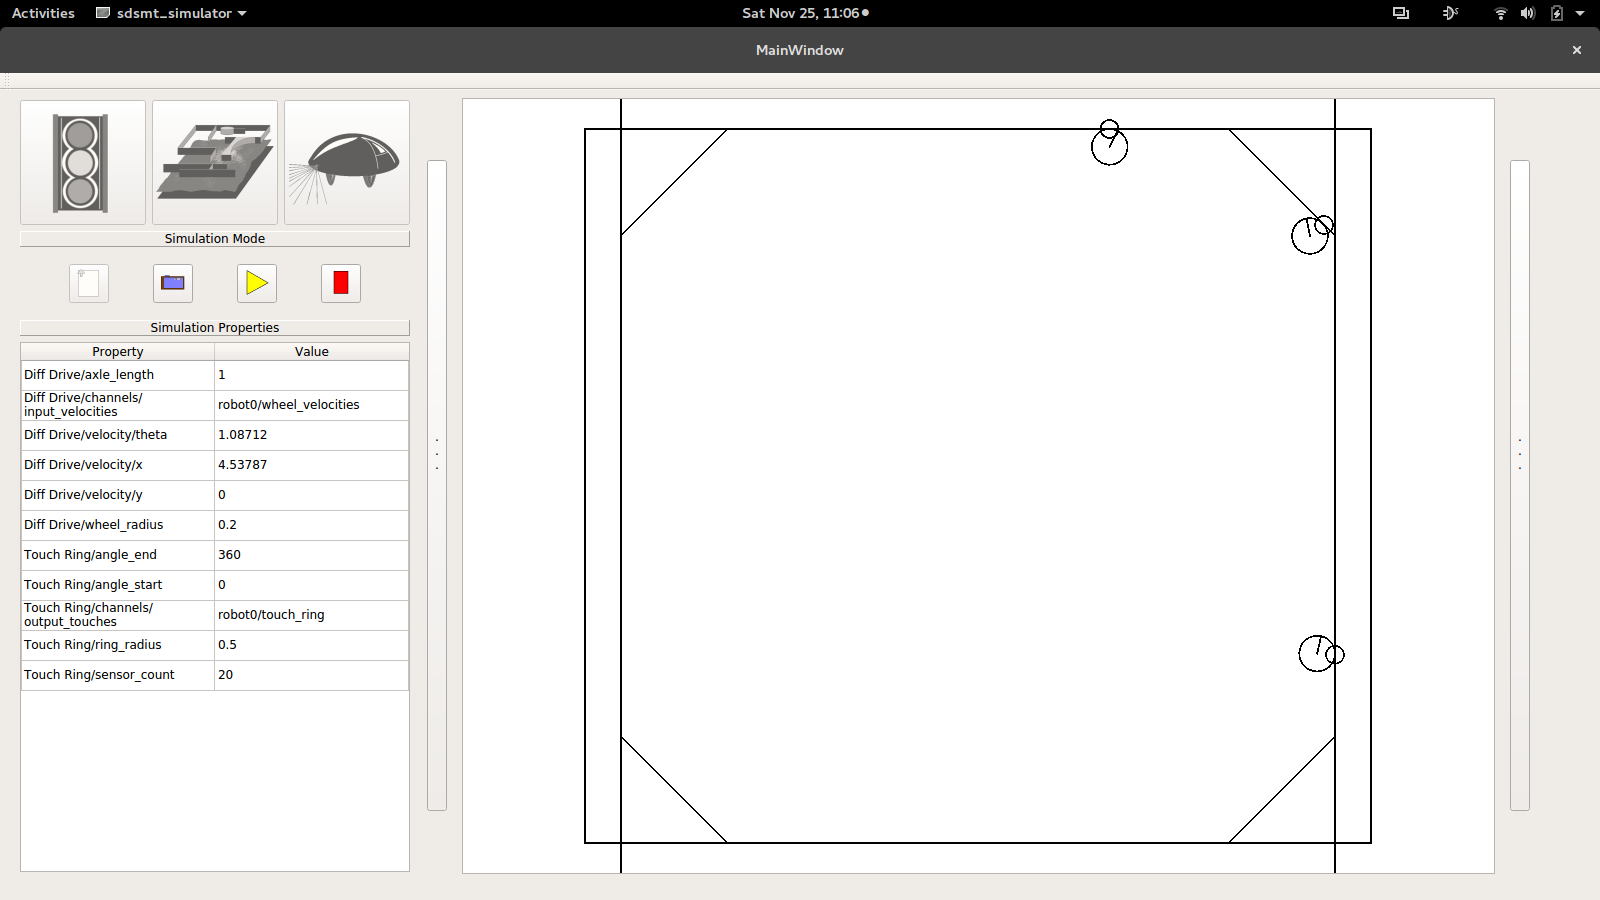
\includegraphics[width=0.75\textwidth]{./Images/Sprint3_hasBox_originalUI}
	\end{center}
	\caption{The MVP of our product, with a loaded map of four squares and three differential drive robots spawned at random locations in various orientations in the world view. \label{mvp1}}
\end{figure}


\subsection{RoboScience Simulator}

The final product, the RoboScience Simulator, improved upon the MVP with many features requested by the client. These included the world object designer, the simulation designer, file loading/saving, image to map loading, improved physics, joystick control, lidar sensor, Ackermann steering, quick save/quick load, time warping, and multiple shapes of robots among other things. We also updated our Box2D version and implemented our software for compatibility with ROS2 and Windows 10 OS. The final product, as pictured below, has a different UI look than the MVP as well. This is due to all new icons and the addition of the menus and components lists on the right hand side disappearing menu. 

\begin{figure}[!htb]
	\begin{center}
		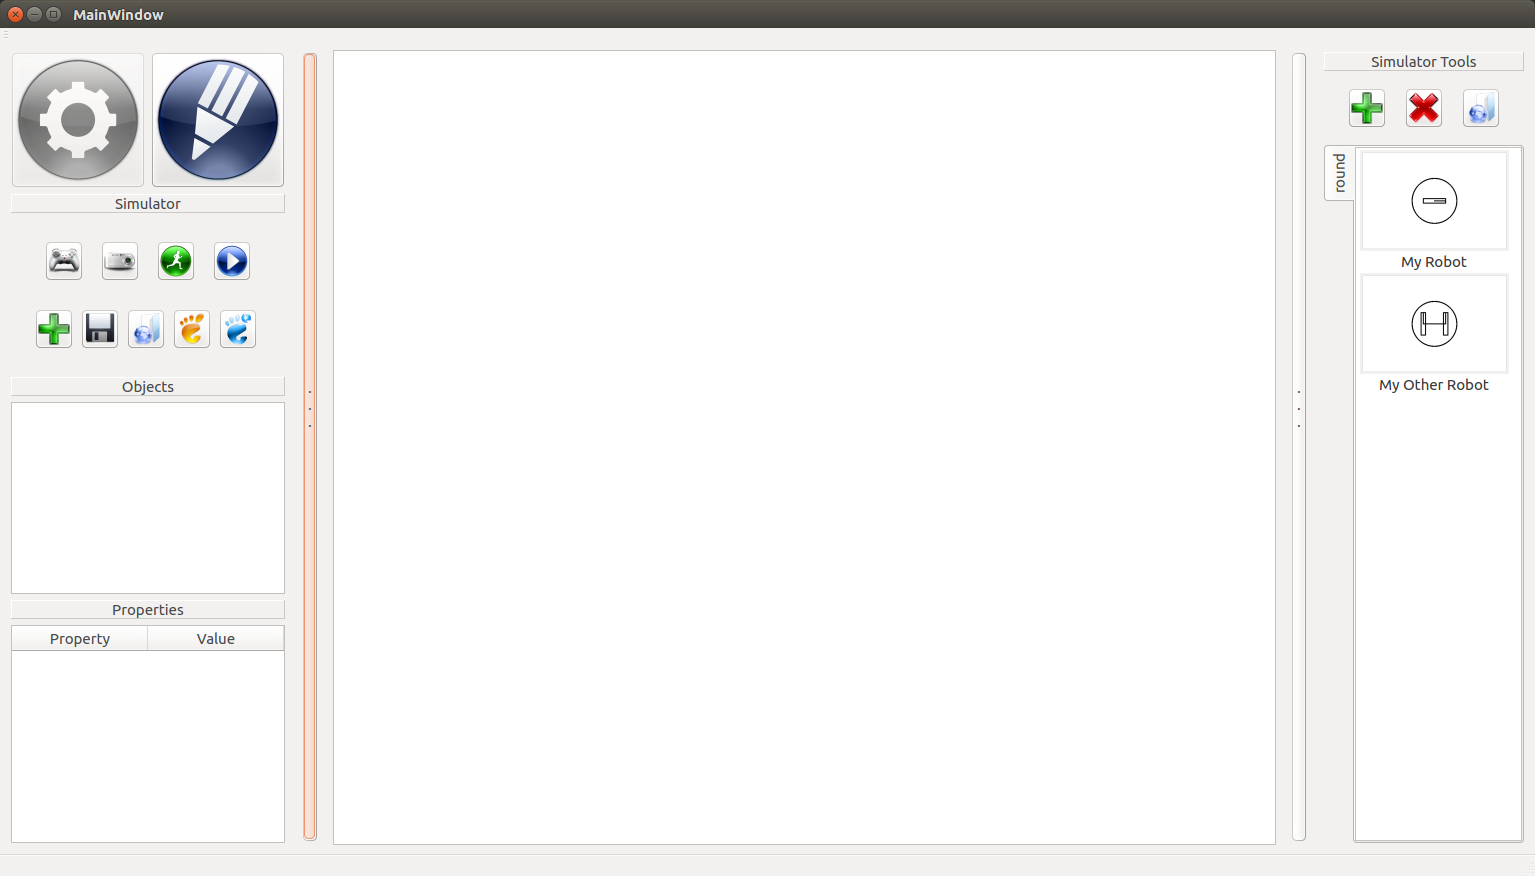
\includegraphics[width=0.75\textwidth]{./Images/simulator_with_my_robots}
	\end{center}
	\caption{The RoboScience Simulator, showing two robots which were constructed in the designer available to be added to the simulation. As shown, there are about twice the number of tool buttons available on the left hand menu. This is due to the added features from the MVP, such as quick save/quick load and joystick controls. \label{mvp2}}
\end{figure}

\begin{figure}[!htb]
	\begin{center}
		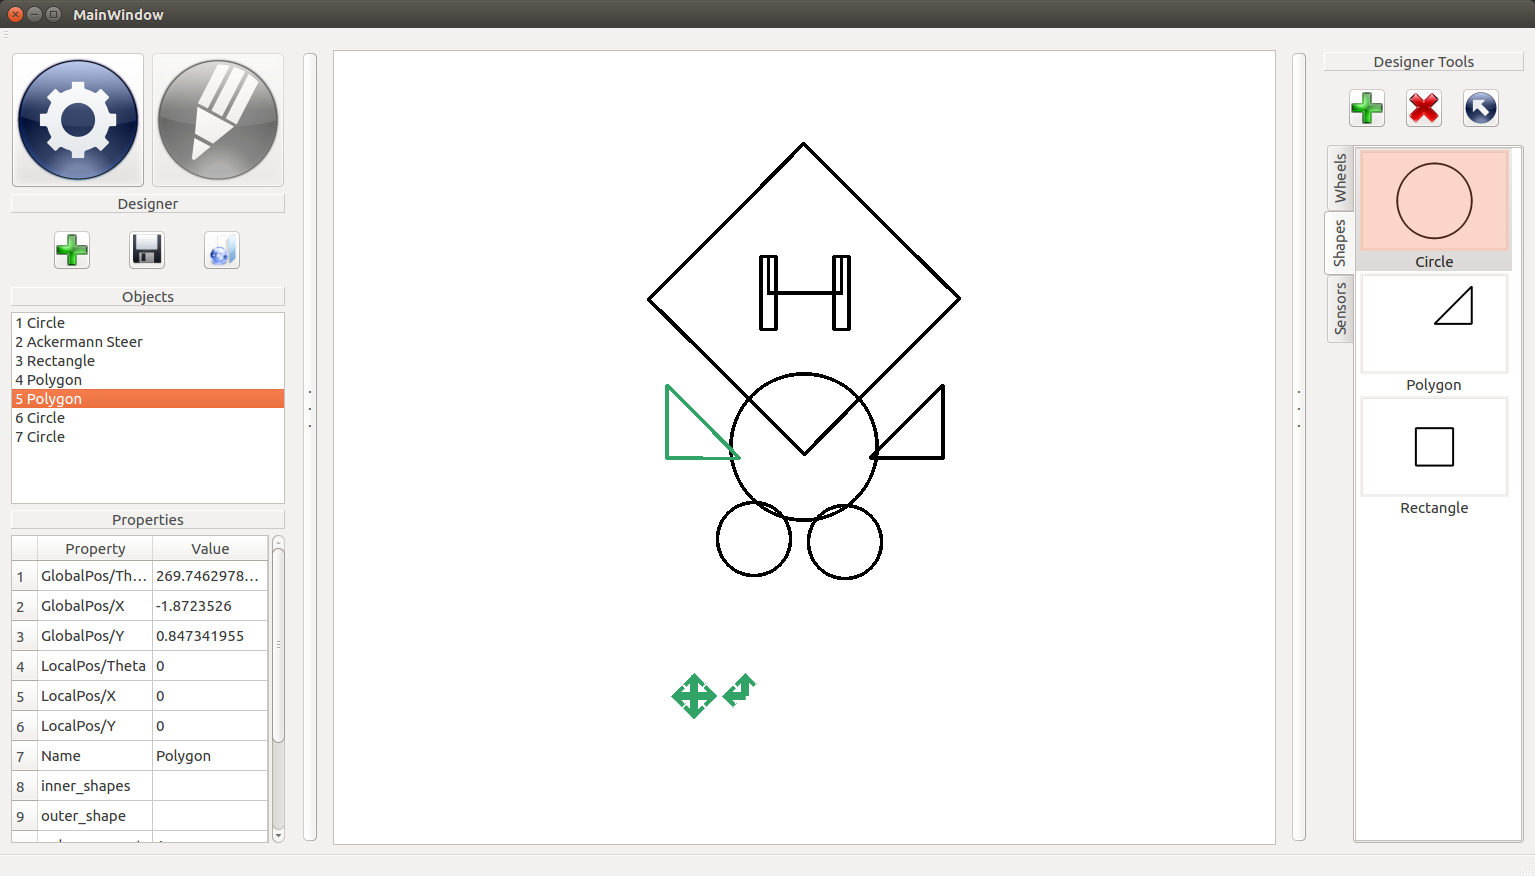
\includegraphics[width=0.75\textwidth]{./Images/designer_weird_robot}
	\end{center}
	\caption{The RoboScience Simulator, showing the construction of a humanoid 2D robot in the designer. Here we see tabs for different "types" of components a user can add. Each component is a plugin and new plugins can be written and included by users if the product doesn't already have what they're looking for. \label{mvp3}}
\end{figure}